%%%%%%%%%%%%%%%%%%%%%%%%%%%%%%%%%%%%%%%%%
% Simple Sectioned Essay Template
% LaTeX Template
%
% This template has been downloaded from:
% http://www.latextemplates.com
%
% Note:
% The \lipsum[#] commands throughout this template generate dummy text
% to fill the template out. These commands should all be removed when 
% writing essay content.
%
%%%%%%%%%%%%%%%%%%%%%%%%%%%%%%%%%%%%%%%%%

%----------------------------------------------------------------------------------------
%	PACKAGES AND OTHER DOCUMENT CONFIGURATIONS
%----------------------------------------------------------------------------------------

\documentclass[12pt]{article} % Default font size is 12pt, it can be changed here

\usepackage{geometry} % Required to change the page size to A4
\geometry{a4paper} % Set the page size to be A4 as opposed to the default US Letter
\usepackage[utf8]{inputenc}

\usepackage{graphicx} % Required for including pictures

\usepackage{float} % Allows putting an [H] in \begin{figure} to specify the exact location of the figure
\usepackage{wrapfig} % Allows in-line images such as the example fish picture

\usepackage{lipsum} % Used for inserting dummy 'Lorem ipsum' text into the template

\linespread{1.2} % Line spacing

%\setlength\parindent{0pt} % Uncomment to remove all indentation from paragraphs

\graphicspath{{Pictures/}} % Specifies the directory where pictures are stored

\begin{document}

%----------------------------------------------------------------------------------------
%	TITLE PAGE
%----------------------------------------------------------------------------------------

\begin{titlepage}

\newcommand{\HRule}{\rule{\linewidth}{0.5mm}} % Defines a new command for the horizontal lines, change thickness here

\center % Center everything on the page

\textsc{\LARGE Universidad Veracruzana}\\[1.5cm] % Name of your university/college
\textsc{\Large Tópicos Selectos de Computación I}\\[0.5cm] % Major heading such as course name


\HRule \\[0.4cm]
{ \huge \bfseries Red Metro}\\[0.4cm] % Title of your document
\HRule \\[1.5cm]

\begin{minipage}{0.4\textwidth}
\begin{flushleft} \large
\emph{Autores:}\\
Lorenzo Alfonso Ramírez Zarate\\
Osvaldo Cordova Aburto\\
Cristian Shaid de Jesús García\\
Alberto Sánchez Ramos % Your name
\end{flushleft}
\end{minipage}
~
\begin{minipage}{0.4\textwidth}
\begin{flushright} \large
\emph{Profesor:} \\
Luis G. Montané Jiménez % Supervisor's Name
\end{flushright}
\end{minipage}\\[4cm]

{\large \today}\\[3cm] % Date, change the \today to a set date if you want to be precise

%\includegraphics{Logo}\\[1cm] % Include a department/university logo - this will require the graphicx package

\vfill % Fill the rest of the page with whitespace

\end{titlepage}

%----------------------------------------------------------------------------------------
%	TABLE OF CONTENTS
%----------------------------------------------------------------------------------------

\tableofcontents% Include a table of contents

\newpage % Begins the essay on a new page instead of on the same page as the table of contents 

%----------------------------------------------------------------------------------------
%	INTRODUCTION
%----------------------------------------------------------------------------------------

\section{Introducción} % Major section

En la actualidad se cuenta con una red de metro en algunas ciudades del mundo, en las cuales se tienen diferentes rutas, estaciones, así como, diferentes horios. 

Es algo complejo lograr aprenderse las diferentes rutas que existen, asi como los diferenes horarios y los transbordos al ir de un lugar a otro, donde la ciudad de origen pertenezca a una ruta diferente de la de la ciudad de destino.
Así, si se es un visitante de alguna ciudad con metro se tendría que revisar toda la información que se necesite en su respectivo momento. Entonces, si se visitan demasiadas ciudades que cuenten con la estación del metro sería demasiado trabajo para una persona con muchas ocupaciones.

Por ello, muchos desarrolladores se han tomado algo de tiempo en desarrollar aplicaciones para la red del metro en su pais, un ejemplo es la red del metro de México la cual cuenta con 12 Rutas con 195 estaciones en total. Algunas aplicaciones en Android disponibles en la Play Store para obtener información del metro son: Metro DF, Cyber Metro, Metro y Metrobus de Mexico, Red transporte DF, Metrodroid DF, entre otras más.

Revisando estas aplicaciones decidimos crear nuestra propuesta de aplicación para redes de metro, pero no sólo crear una similar sino aplicar algoritmia que consideramos que será útil en este problema y que observamos que las otras aplicaciones no utilizaban. Esta algoritmia nos ayudará a interpretar ciertos contextos que puedan afectar la afluencia del metro.

Lo que se plantea es que se pueda utilizar esta propuesta de aplicación no sólo en esta red de metro, sino en las redes de metros de otras ciudades. Aunque por el momento utilizaremos datos de la red de metro del DF.
\pagebreak

\section{Propuesta} % Major section
%------------------------------------------------

\subsection{Arquitectura General del Sistema} % Sub-section
\begin{center}
	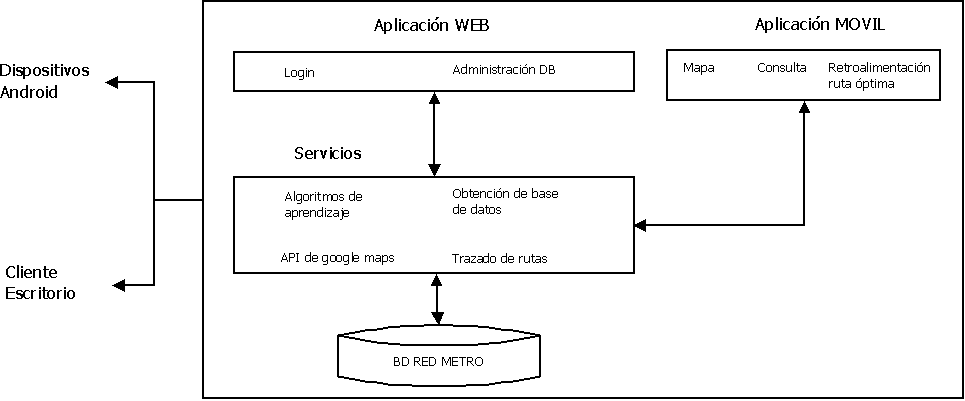
\includegraphics[width = 15cm]{Arquitectura_sistema}
\end{center}
\pagebreak

\section{Diagrama de Componentes} % Major section

\begin{center}
	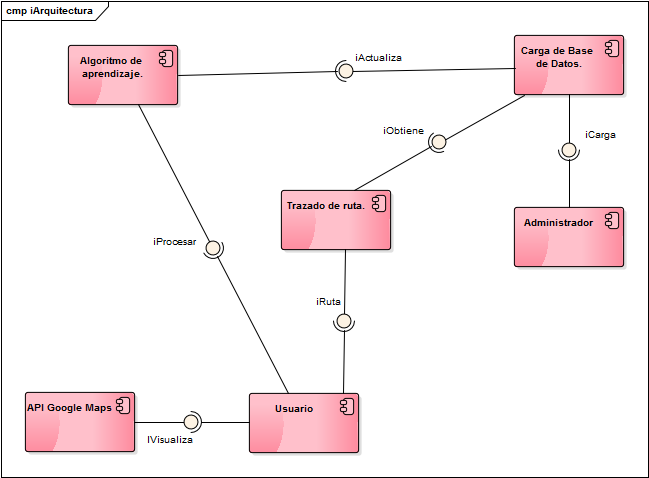
\includegraphics[width = 15cm]{ModeloDeComponentes}
\end{center}
\pagebreak

%------------------------------------------------

\subsection{Proceso de Recuperación de Información} % Sub-section

El sistema será alimentado por los clientes (administradores) a los que se les dará acceso a la parte administrativa WEB donde deberán cargar su información a partir de unos archivos de Excel con la descripción de las rutas y los horarios.

El sistema proporciona unas plantillas para las rutas y los horarios con un formato que deberá ser respetado para la recuperación de información, en caso de no ser respetado el formato, el sistema no permitirá subir la información a la base de datos.

El proceso a seguir es:	\\
\begin{itemize}
\item Los clientes (administradores) se ponen en contacto con los desarrolladores de la aplicación.

\item Los desarrolladores le proporcionan una cuenta de acceso para la aplicación Web.

\item Los Clientes (administradores) bajan la plantilla de rutas y horarios.

\item Los Clientes (administradores) llenan las plantillas y las suben al sistema.

\item El sistema valida que la información sea correcta y que cumpla con aspectos de seguridad mínimos (SQL Injection), de no ser así, se muestra un mensaje de alerta informando al usuario que la carga de datos ha fallado.

\item El sistema procesa el archivo de Excel a formato JSON para después ser manipulado con un script de Python y realizar la inserción de información a la base de datos.
\end{itemize}
\pagebreak


%------------------------------------------------
\section{Modelo Relacional de la Base de Datos} % Major section

La base de datos sólo contiene información de las rutas, y los horarios. No llevan relación porque son considerados como simples catálogos en donde los horarios son siempre iguales para cada país.\\

\begin{center}
	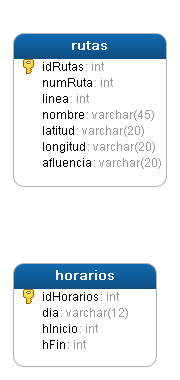
\includegraphics[width = 7cm]{Modelo_Relacional}
\end{center}
\pagebreak

\subsection{Avance de la Plataforma (Implementación, Servicios, etc...)}


Los datos de las rutas y los horarios de la red de metro de México fueron cargados a la base de datos “RedMetro”.



%----------------------------------------------------------------------------------------
%	MAJOR SECTION X - TEMPLATE - UNCOMMENT AND FILL IN
%----------------------------------------------------------------------------------------

%\section{Content Section}

%\subsection{Subsection 1} % Sub-section

% Content

%------------------------------------------------

%\subsection{Subsection 2} % Sub-section

% Content

%----------------------------------------------------------------------------------------
%	CONCLUSION
%----------------------------------------------------------------------------------------


%----------------------------------------------------------------------------------------
%	BIBLIOGRAPHY
%----------------------------------------------------------------------------------------

%\begin{thebibliography}{99} % Bibliography - this is intentionally simple in this template

%\bibitem[Figueredo and Wolf, 2009]{Figueredo:2009dg}
%Figueredo, A.~J. and Wolf, P. S.~A. (2009).
%\newblock Assortative pairing and life history strategy - a cross-cultural
%  study.
%\newblock {\em Human Nature}, 20:317--330.
 
%\end{thebibliography}

%----------------------------------------------------------------------------------------

\end{document}